\documentclass[12pt,a4paper, dvipsnames]{article}

\usepackage{amsmath}   				% Math environments (equation, align, ..)
\usepackage{graphicx}  				% Including pictures (includegraphics, ...)
\usepackage{tabularx} 				% Table
\usepackage{siunitx} 				% \si command
\usepackage[hidelinks]{hyperref}	% For linked table of contents (toc)
\newlength\tindent 					% Rename parident to tindent
\setlength{\tindent}{\parindent}	
\setlength{\parindent}{0pt} 		% Disable indent
\usepackage[skip=-1em]{caption} 	% Reduce distance between image and caption
\renewcommand{\labelitemi}{$-$}		% Less space between items in itemize env
\setcounter{MaxMatrixCols}{20} 		% Set \begin{matrix} to max 20 columns


% Toggle between text and slide mode
\def \makeSlides {}
%-------------------%
\ifx \makeSlides\defined
	\usepackage[left=2cm, right=2cm, top=2cm,bottom=2cm]{geometry} % Set page margins	
\else
	\usepackage{02_design/slides}	% Use slide format template (sets xcolor)
\fi
%-------------------%


% Facilitate writing
\input{00_sections/11_ownCommands/ownCommands}





\begin{document}
	\tableofcontents
	\clearpage
	
	\section{Control Design}
\subsection{Methodology}
\begin{enumerate}
	\item Study the system (plant) to be controlled and obtain initial information about the control objectives
	\item Model the system and simplify the model, if necessary
		\begin{enumerate}
			\item Identification of the input and output variables of the process
			\item Identify the dependencies of each variable, starting with the output, until the system only depends on input variables
			\item Identify the transmission behaviour between the signals
		\end{enumerate}
	\item Scale the variables and analyze the resulting model; determine its properties
	\item Decide which variables are to be controlled (controlled outputs)
	\item Decide on the measurements and manipulated variables: what sensors and actuators will be used and where will they be placed?
	\item Select the control configuration
	\item Decide on the type of controller to be used
	\item Decide on performance specifications, based on the overall control objectives
	\item Design a controller
	\item Analyze the resulting controlled system to see if the specifications are satisfied; and if they are not satisfied modify the specificiations or the type of controller
	\item Simulate the resulting controlled system, either on a computer or a pilot plant
	\item Repeat from step 2, if necessary
	\item Choose hardware and software and implement the controller
	\item Test and validate the control system, and tune the controller on-line, if necessary
\end{enumerate}



		
\subsection{Control Objectives}
1. Tilt control \\
2. Height control 
\clearpage

\subsection{System Model}
\begin{figure}[htb!]
	\centering
	\includegraphics[width=0.7\textwidth]{01_figures/intro_basicSystem}
	\caption{Basic system structure}
	\label{fig:intro_basicSystem}
\end{figure}
\clearpage

\begin{figure}[htb!]
	\centering
	
\includegraphics[width=0.5\textwidth]{01_figures/intro_cosChoice}
	\caption{Choice of coordinate system}
	\label{fig:intro_cos}
\end{figure}

Geodetical x,y,z-position
\begin{align*}
	\vec{x} &= \begin{pmatrix} x \\	y \\ z \end{pmatrix}
\intertext{Absolute velocity in x,y,z-direction of the body frame}
	\vec{v} &= \begin{pmatrix} u \\ v \\ w \end{pmatrix}
\intertext{Euler Angles}
	\vec{\Phi} &= \begin{pmatrix} \Phi \\ \Theta \\ \Psi \end{pmatrix}
\intertext{Rotational speed around x,y,z-axis of the body frame}
	\vec{\omega} &= \begin{pmatrix} p \\ q \\ r \end{pmatrix}
\intertext{PWM signal for electronic speed controller (ESC)}
	\vec{u} &= \begin{pmatrix} PWM_1 \\ PWM_2 \\ PWM_3 \\ PWM_4 \end{pmatrix}
\end{align*}

Absolute speed in body frame transformed to inertial frame yields derivative of geodatic coordinates
\begin{align*}
	\dot{\vec{x}} &= \underline{T}_b^i \cdot \vec{v}
\intertext{Principle of linear momentum of point mass - body fixed frame}
	\frac{\text{d}\vec{p}}{\text{d}t} &= \sum \vec{F} 
	\\
	m \cdot \frac{\text{d}\vec{v}}{\text{d}t} &=\sum \vec{F}
	\\
	m \cdot \left(\frac{\text{d}\vec{v}}{\text{d}t}\right)_{\omega=0} +  \vec{\omega} \times m \cdot\vec{v} &=\sum \vec{F}
	\\ \Rightarrow \dot{\vec{v}} &= \frac{1}{m} \cdot \sum \vec{F} - \vec{\omega} \times \vec{v}	
\intertext{with (see Eq.~\ref{eq:Tib} for $\underline{T}_i^b$)}
	\sum \vec{F} &= \underline{T}_i^b \cdot \begin{pmatrix} 0 \\ 0 \\ -m\cdot g	\end{pmatrix} + \begin{pmatrix} 0 \\ 0 \\ F_1 + F_2 + F_3 + F_4	\end{pmatrix}
\intertext{Angular velocities in body frame can be transformed to the derivatives of the euler angles via the Kalman transformation matrix (see Eq.~\ref{eq:Vbi} for $\underline{V}_b^i$)}
	\dot{\vec{\Phi}} &= \underline{V}_b^i \cdot \vec{\omega}
\intertext{Principle of momentum - body fixed frame}
	\frac{\text{d}L}{\text{d}t} &= \sum \vec{M}
	\\
	\left(\frac{\text{d}L}{\text{d}t}\right)_{\omega=0} + \vec{\omega} \times L &= \sum \vec{M}
	\\
	\inertia \cdot \left(\frac{\text{d}\vec{\omega}}{\text{d}t}\right)_{\omega=0} + \vec{\omega} \times \left( \inertia \cdot \vec{\omega} \right) &= \sum \vec{M} 
	\\
	\Rightarrow \dot{\vec{\omega}} &= \inertia^{-1} \cdot \left( \sum \vec{M} - \vec{\omega} \times \left( \inertia \cdot \vec{\omega} \right) \right)
\intertext{with}
	\sum \vec{M} &= \begin{pmatrix} l\cdot(F_2 - F_4) \\ l\cdot(F_3 - F_1) \\ M_1 - M_2 + M_3 - M_4 \end{pmatrix}
\intertext{The general state space  $\dot{x} = f(\vec{x}, \vec{u})$ therefore looks as follows}
		 \begin{pmatrix} \dot{\vec{x}} \\ \dot{\vec{v}} \\ \dot{\vec{\Phi}} \\ \dot{\vec{\omega}} \end{pmatrix}&= \begin{pmatrix}
	\underline{T}_b^i \cdot v 
	\\[0.8em]
	\underline{T}_i^b \cdot \begin{pmatrix}0\\0\\-g	\end{pmatrix} + \begin{pmatrix}0\\0\\ \frac{1}{m}\sum_{i=1}^4 F_i(\ctrl{i})	\end{pmatrix} - \vec{\omega} \times v 
	\\[2em]
	\underline{V}_b^i \cdot \omega
	\\[0.8em]
	\inertia^{-1} \cdot \left( \begin{pmatrix} l \cdot \left(F_2(\ctrl{2}) - F_4(\ctrl{4} \right)  \\ l \cdot \left(F_3(\ctrl{3}) - F_1(\ctrl{1} \right)  \\ \sum_{i=1}^4 (-1)^{i+1} \cdot M(\ctrl{i}) \end{pmatrix} - \vec{\omega} \times \left( \inertia \cdot \vec{\omega} \right) \right)
	\end{pmatrix}
\end{align*}

For a quadrotor frame symmetric to the x- and y-axis, the inertia elements $\inertiaii{12}=\inertiaii{21}$ and $\inertiaii{23}=\inertiaii{32}$ equal 0. With
\begin{align}
	\vec{\omega} \times \left(\inertia \cdot \vec{\omega} \right) &= \begin{pmatrix}
		\left(\Theta_{b31} \cdot \omega_1 + \Theta_{b32} \cdot \omega_2 + \Theta_{b33} \cdot \omega_3 \right) \cdot \omega_2 - \left(\Theta_{b21} \cdot \omega_1 + \Theta_{b22} \cdot \omega_2 + \Theta_{b23} \cdot \omega_3 \right) \cdot \omega_3  
	\\[0.5em]
		\left(\Theta_{b11} \cdot \omega_1 + \Theta_{b12} \cdot \omega_2 + \Theta_{b13} \cdot \omega_3 \right) \cdot \omega_3 - \left(\Theta_{b31} \cdot \omega_1 + \Theta_{b32} \cdot \omega_2 + \Theta_{b33} \cdot \omega_3 \right) \cdot \omega_1 
	\\[0.5em]
		\left(\Theta_{b21} \cdot \omega_1 + \Theta_{b22} \cdot \omega_2 + \Theta_{b23} \cdot \omega_3 \right) \cdot \omega_1 - \left(\Theta_{b11} \cdot \omega_1 + \Theta_{b12} \cdot \omega_2 + \Theta_{b13} \cdot \omega_3 \right) \cdot \omega_2
	\end{pmatrix} \nonumber
	\\
	&= \begin{pmatrix}  
		\left(\inertiaii{31} \cdot \omega_1 + \inertiaii{33} \cdot \omega_3 \right) \cdot \omega_2 - \inertiaii{22} \cdot \omega_2 \cdot \omega_3  
	\\[0.5em]
		\left(\inertiaii{11} \cdot \omega_1 + \inertiaii{13} \cdot \omega_3 \right) \cdot \omega_3 - \left(\inertiaii{31} \cdot \omega_1 + \inertiaii{33} \cdot \omega_3 \right) \cdot \omega_1 
	\\[0.5em]
		\inertiaii{22} \cdot \omega_2 \cdot \omega_1 - \left(\inertiaii{11} \cdot \omega_1 + \inertiaii{13} \cdot \omega_3 \right) \cdot \omega_2
	\end{pmatrix} \nonumber
\intertext{and the resulting simplifications of the inverse of the inertia matrix (see section~\ref{subsec:InertiaMatrix}) the state space can be stated as follows}
	\Rightarrow \begin{pmatrix}  \dot{x} \\ \dot{y} \\ \dot{z} \\ \dot{u} \\ \dot{v} \\ \dot{w} \\ \dot{\Phi} \\ \dot{\Theta} \\ \dot{\Psi} \\ \dot{p} \\ \dot{q} \\ \dot{r} \end{pmatrix} &= \begin{pmatrix}
		\Tbirc \cdot u + (\Tbircc) \cdot v + \left(\Tbirccc \right) \cdot w \\[0.5em]
		\Tbirrc \cdot u + (\Tbirrcc) \cdot v + \left( \Tbirrccc \right) \cdot w \\[0.5em]
		\Tbirrrc \cdot u + \left(\Tbirrrcc \right) \cdot v + \left( \Tbirrrccc \right) \cdot w \\[0.5em]
		-g \cdot \Tibrccc - \omega_2 \cdot w + \omega_3 \cdot v	\\[0.5em]
		-g \cdot \Tibrrccc - \omega_3 \cdot u + \omega_1 \cdot w \\[0.5em]
		-g \cdot \Tibrrrccc - \omega_1 \cdot v + \omega_2 \cdot u + \frac{1}{m} \cdot \left( F_1(\ctrl{1}) + F_2(\ctrl{2}) + F_3(\ctrl{3}) + F_4(\ctrl{4}) \right)
		\\[0.5em]
		p + q \cdot \Vbircc + r \cdot \Vbirccc \\[0.5em]
		q \cdot \Vbirrcc + r \cdot \Vbirrccc \\[0.5em]
		q \cdot \Vbirrrcc + r \cdot \Vbirrrccc 
		\\[0.5em]
		\begin{pmatrix}
		\dfrac{\inertiaii{33}}{\inertiaii{11} \cdot \inertiaii{33} - \inertiaii{13}^2} & 0 & -\dfrac{\inertiaii{13}}{\inertiaii{11} \cdot \inertiaii{33} - \inertiaii{13}^2} \\
		0  & \dfrac{1}{\inertiaii{22}} & 0 \\
		-\dfrac{\inertiaii{13}}{\inertiaii{11} \cdot \inertiaii{33} - \inertiaii{13}^2} & 0 & \dfrac{\inertiaii{11}}{\inertiaii{11} \cdot \inertiaii{33} - \inertiaii{13}^2}
		\end{pmatrix}
		\cdot 
		\begin{pmatrix} l\cdot(F_2 - F_4) - \left(\Theta_{b31} \cdot \omega_1 + \Theta_{b33} \cdot \omega_3 \right) \cdot \omega_2 + \Theta_{b22} \cdot \omega_2 \cdot \omega_3  
		\\[0.5em]
		l\cdot(F_3 - F_1) - \left(\Theta_{b11} \cdot \omega_1 + \Theta_{b13} \cdot \omega_3 \right) \cdot \omega_3 + \left(\Theta_{b31} \cdot \omega_1 + \Theta_{b33} \cdot \omega_3 \right) \cdot \omega_1 
		\\[0.5em]
		M_1 - M_2 + M_3 - M_4 - \Theta_{b22} \cdot \omega_2 \cdot \omega_1 + \left(\Theta_{b11} \cdot \omega_1 +  \Theta_{b13} \cdot \omega_3 \right) \cdot \omega_2
		\end{pmatrix}
	\end{pmatrix}
\end{align}
\clearpage

The esc's and bldc is identified using following input sequence and resulting force.

\begin{figure}[htb!]
	\centering
	\includegraphics[width=0.7\textwidth]{01_figures/mdl_bldcIdent}
	\caption{ESC + BLDC Unit - Measured input output behaviour}
	\label{fig:mdl_bldcIdent}
\end{figure}

\begin{figure}[htb!]
	\centering
	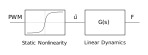
\includegraphics[width=0.6\textwidth]{01_figures/mdl_hammerstein}
	\caption{Hammerstein model structure}
	\label{fig:mdl_hammerstein}
\end{figure}

Assuming a Hammerstein model structure (see Fig.~\ref{fig:mdl_hammerstein}) the input force to the quadrotor model is based on the following model structure:
\begin{align*}
	\dot{F} &= A_{hammerstein} \cdot F + B_{hammerstein} \cdot \tilde{u} \\[0.5em]
	\tilde{u} &= f(\text{PWM}) 
	\\[1em]
	\Rightarrow F &= \dfrac{b_0}{a_0 - a_1 \cdot z^{-1}} \cdot \tilde{u} \\[0.5em]
	\tilde{u} &= p_3 \cdot \ctrl{\text{PWM}}^3 + p_2 \cdot \ctrl{\text{PWM}}^2 + p_1 \cdot \ctrl{\text{PWM}} + p_0
\intertext{For the purpose of control design, the dynamics are assumed sufficiently fast and only the nonlinearity is considered. The static gain of the transfer function for a step response is}
	K &= \dfrac{b_0}{a_0 - a_1}
\end{align*}
\clearpage

\subsection{Model Analysis}
Analyze linearized model around setpoint $\vec{x}_0 = \begin{pmatrix} x_0 & y_0 & z_0 & \vec{0} \end{pmatrix}^T $ and $\vec{F}_0 = \begin{pmatrix} \frac{m\cdot g}{4} & \frac{m\cdot g}{4} & \frac{m\cdot g}{4} & \frac{m\cdot g}{4} \end{pmatrix}^T$
\begin{align*}
\dot{x}_0 &= \vec{0}
	\\
	A &= \begin{pmatrix}
		0 & 0 & 0 	& 1 & 0 & 0 	& 0 & 0 & 0 	& 0 & 0 & 0
	\\
		0 & 0 & 0 	& 0 & 1 & 0 	& 0 & 0 & 0 	& 0 & 0 & 0
	\\
		0 & 0 & 0 	& 0 & 0 & 1 	& 0 & 0 & 0 	& 0 & 0 & 0
	\\
		0 & 0 & 0 	& 0 & 0 & 0 	& 0 & g & 0 	& 0 & 0 & 0
	\\
		0 & 0 & 0 	& 0 & 0 & 0 	& -g & 0 & 0 	& 0 & 0 & 0
	\\
		0 & 0 & 0 	& 0 & 0 & 0 	& 0 & 0 & 0 	& 0 & 0 & 0
	\\
		0 & 0 & 0 	& 0 & 0 & 0 	& 0 & 0 & 0 	& 1 & 0 & 0
	\\
		0 & 0 & 0 	& 0 & 0 & 0 	& 0 & 0 & 0 	& 0 & 1 & 0
	\\
		0 & 0 & 0 	& 0 & 0 & 0 	& 0 & 0 & 0 	& 0 & 0 & 1
	\\
		0 & 0 & 0 	& 0 & 0 & 0 	& 0 & 0 & 0 	& 0 & 0 & 0
	\\
		0 & 0 & 0 	& 0 & 0 & 0 	& 0 & 0 & 0 	& 0 & 0 & 0
	\\
		0 & 0 & 0 	& 0 & 0 & 0 	& 0 & 0 & 0 	& 0 & 0 & 0
	\end{pmatrix}
	\\
	\vec{B} &= \begin{pmatrix} 
	0 & 0 & 0 & 0 \\
	0 & 0 & 0 & 0 \\
	0 & 0 & 0 & 0 \\
	0 & 0 & 0 & 0 \\
	0 & 0 & 0 & 0 \\
	\frac{1}{m} & \frac{1}{m} & \frac{1}{m} & \frac{1}{m} \\
	0 & 0 & 0 & 0 \\
	0 & 0 & 0 & 0 \\
	-\dfrac{\inertiaii{13}}{\inertiaii{11} \cdot \inertiaii{33} - \inertiaii{13}^2} \cdot \dfrac{\text{d}M_1}{\text{d}F_1} & \dfrac{\inertiaii{33}\cdot l + \inertiaii{13} \cdot \frac{\text{d}M_2}{\text{d}F_2} }{\inertiaii{11} \cdot \inertiaii{33} - \inertiaii{13}^2}  & -\dfrac{\inertiaii{13}}{\inertiaii{11} \cdot \inertiaii{33} - \inertiaii{13}^2} \cdot \dfrac{\text{d}M_3}{\text{d}F_3} & \dfrac{-\inertiaii{33}\cdot l + \inertiaii{13} \cdot \frac{\text{d}M_4}{\text{d}F_4} }{\inertiaii{11} \cdot \inertiaii{33} - \inertiaii{13}^2} 
	\\
	-\dfrac{l}{\Theta_{22}} & 0 & \dfrac{l}{\Theta_{22}} & 0
	\\
	\dfrac{\inertiaii{11}}{\inertiaii{11} \cdot \inertiaii{33} - \inertiaii{13}^2} \cdot \dfrac{\text{d}M_1}{\text{d}F_1} & \dfrac{-\inertiaii{13}\cdot l - \inertiaii{11} \cdot \frac{\text{d}M_2}{\text{d}F_2} }{\inertiaii{11} \cdot \inertiaii{33} - \inertiaii{13}^2} & \dfrac{\inertiaii{11}}{\inertiaii{11} \cdot \inertiaii{33} - \inertiaii{13}^2} \cdot \dfrac{\text{d}M_3}{\text{d}F_3} & \dfrac{\inertiaii{13}\cdot l - \inertiaii{11} \cdot \frac{\text{d}M_4}{\text{d}F_4} }{\inertiaii{11} \cdot \inertiaii{33} - \inertiaii{13}^2}
	\end{pmatrix}
\end{align*}
Tilt, orientation and height dynamics ($\Phi,~\Theta,~\Psi,~z$) are decoupled from remaining system. Only x and y direction are coupled to pitch and roll angles.
\clearpage

\subsection{Controlled Outputs}
The control goal is to keep a stable tilt and fixed height ($\Phi,~\Theta,~z$). As these states are decoupled from the rest, the reduced model 
\begin{align}
	\dot{x}_{red} &= \begin{pmatrix} 0 & 0 & 0 & 1 & 0 & 0 \\
									 0 & 0 & 0 & 0 & 1 & 0 \\
									 0 & 0 & 0 & 0 & 0 & 1 \\
									 0 & 0 & 0 & 0 & 0 & 0 \\
									 0 & 0 & 0 & 0 & 0 & 0 \\
									 0 & 0 & 0 & 0 & 0 & 0 
					 \end{pmatrix} \cdot \vec{x}_{red} + 
					 \begin{pmatrix}
					 	0 & 0 & 0 & 0 \\
					 	0 & 0 & 0 & 0 \\
					 	0 & 0 & 0 & 0 \\
					 	\frac{1}{m} & \frac{1}{m} & \frac{1}{m} & \frac{1}{m} \\
					 	-\dfrac{\inertiaii{13}}{\inertiaii{11} \cdot \inertiaii{33} - \inertiaii{13}^2} \cdot \dfrac{\text{d}M_1}{\text{d}F_1} & \dfrac{\inertiaii{33}\cdot l + \inertiaii{13} \cdot \frac{\text{d}M_2}{\text{d}F_2} }{\inertiaii{11} \cdot \inertiaii{33} - \inertiaii{13}^2}  & -\dfrac{\inertiaii{13}}{\inertiaii{11} \cdot \inertiaii{33} - \inertiaii{13}^2} \cdot \dfrac{\text{d}M_3}{\text{d}F_3} & \dfrac{-\inertiaii{33}\cdot l + \inertiaii{13} \cdot \frac{\text{d}M_4}{\text{d}F_4} }{\inertiaii{11} \cdot \inertiaii{33} - \inertiaii{13}^2} 
					 	\\
					 	-\dfrac{l}{\Theta_{22}} & 0 & \dfrac{l}{\Theta_{22}} & 0
					 \end{pmatrix} \cdot \vec{F} \label{eq:mdl_linearized}
\end{align}
with $\vec{x}_{red} = \begin{pmatrix} z, \Phi, \Theta, \dot{z}, p, q \end{pmatrix}^T$ can be treated.
\clearpage

\subsection{Measured and Manipulated Variables}
Add overview of sensor and actuator placement. 
\begin{table}[htb!]
	\centering
	\begin{tabular}{c@{\quad}|c@{\quad}}
		\hline
		\rule{0pt}{12pt} 
		System Inputs & System Outputs
		\\[2pt]
		\hline\rule{0pt}{12pt} 
		$\text{PWM}_\text{esc,1}$ & $\der{u}$ \\
		$\text{PWM}_\text{esc,2}$ & $\der{v}$ \\
		$\text{PWM}_\text{esc,3}$ & $\der{w}$ \\
		$\text{PWM}_\text{esc,4}$ & $p$ \\
		& $q$ \\
		& $r$ \\
		\hline
	\end{tabular}
	\vspace{6mm}
	\caption{Inputs and outputs} 
	\label{tab:mdl_gcai_paramSim}
\end{table}
\clearpage

\subsection{Control Configuration}
\begin{figure}[htb!]
	\centering
	\includegraphics[width=0.7\textwidth]{01_figures/controlStructure}
	\caption{Control structure}
	\label{fig:controlStructure}
\end{figure}
\clearpage
\clearpage

\subsection{Controller Type}
LQR + Kalman Filter.
\clearpage

\subsection{Performance Specification}
Tilt of quadrotor remains unchanged. 
\clearpage

\subsection{Controller - PD}
By reformulating Eq.~\ref{eq:mdl_linearized} as
\begin{align*}
\dot{x}_{red} &= \begin{pmatrix} 0 & 0 & 0 & 1 & 0 & 0 \\
	0 & 0 & 0 & 0 & 1 & 0 \\
	0 & 0 & 0 & 0 & 0 & 1 \\
	0 & 0 & 0 & 0 & 0 & 0 \\
	0 & 0 & 0 & 0 & 0 & 0 \\
	0 & 0 & 0 & 0 & 0 & 0 
\end{pmatrix} \cdot \vec{x}_{red} +
\begin{pmatrix}
	0   \\
	0   \\
	0   \\
	u_1 \\
	u_2 \\
	u_3 
\end{pmatrix}
\\[1em]
\begin{pmatrix} u_1 \\ u_2 \\ u_3 \end{pmatrix} &= 
\begin{pmatrix}
	\frac{1}{m} & \frac{1}{m} & \frac{1}{m} & \frac{1}{m} \\
	-\dfrac{\inertiaii{13}}{\inertiaii{11} \cdot \inertiaii{33} - \inertiaii{13}^2} \cdot \dfrac{\text{d}M_1}{\text{d}F_1} & \dfrac{\inertiaii{33}\cdot l + \inertiaii{13} \cdot \frac{\text{d}M_2}{\text{d}F_2} }{\inertiaii{11} \cdot \inertiaii{33} - \inertiaii{13}^2}  & -\dfrac{\inertiaii{13}}{\inertiaii{11} \cdot \inertiaii{33} - \inertiaii{13}^2} \cdot \dfrac{\text{d}M_3}{\text{d}F_3} & \dfrac{-\inertiaii{33}\cdot l + \inertiaii{13} \cdot \frac{\text{d}M_4}{\text{d}F_4} }{\inertiaii{11} \cdot \inertiaii{33} - \inertiaii{13}^2} 
	\\
	-\dfrac{l}{\Theta_{22}} & 0 & \dfrac{l}{\Theta_{22}} & 0
\end{pmatrix} \cdot \vec{F}
\\[0.5em]
&= E \cdot \vec{F}
\end{align*}
the controller can be designed by interpreting three independant SISO systems: 
\begin{align*}
	\ddot{x}_{i,red}  &= u_i \qquad i=1\text{-}3
\intertext{Choosing a PD controller}
	\ddot{x}_{i,red} + k_d \cdot \dot{x}_{i,red} + k_p \cdot x_{i,red}  &= 0
\intertext{the system's poles can directly prescribed by}
	s_{1/2} &= -\dfrac{k_d}{2} \pm \sqrt{ \left( \dfrac{k_d}{2} \right)^2 - k_p }
\end{align*}
In order to invert $E\cdot \vec{F}$, a further condition can be added by $\sum M_i = 0$ leading to $\begin{pmatrix} 1 & -1 & 1 &-1 \end{pmatrix}$.
\clearpage

\subsection{Controller - LQR}

\clearpage

\subsection{Controller - Kalman filter}
. 
Show observer simulation results and results based on measurement data (in comparison to madgwick).
\clearpage

\subsection{Closed loop simulation}
 Show closed loop control results. State feedback gains, Q, R. 
	
		
	\appendix
	\section{Moving Coordinate Systems}


Derivative of vectors in rotating coordinate systems:
\begin{align}
	\der{\vec{\rho}} &= \vec{\omega} \times \vec{\rho} + \left(\frac{\partial \vec{\rho}}{\partial t} \right)_{\omega=0} \label{eq:a_abs}
\intertext{Absolute velocity and acceleration of a moving point in a moving and rotating coordinate system:}
	\vec{r} &= \vec{r_0} + \vec{\rho} \label{eq:r} \\
	\der{\vec{r}} &= \der{\vec{r_0}} + \vec{\omega} \times \vec{\rho} + v_{rel} \label{eq:der_r} \\
	\dder{\vec{r}} &= \underbrace{ \dder{\vec{r}_0} + \dot{\vec{\omega}} \times \vec{\rho} + \vec{\omega} \times ( \vec{\omega} \times \vec{\rho}) }_{Leading~Acceleration} + \underbrace{2 \vec{\omega} \times v_{rel}}_{\substack{Coriolis\\ Acceleration}} + a_{rel} \label{eq:dder_r}
\end{align}

Notes
\begin{itemize}
	\item Eq.~\ref{eq:dder_r} helps formulate simpler correlations for acceleration of moving points in moving and rotating coordinate systems
	\item For known trajectories (e.g. circular paths), Eq.~\ref{eq:dder_r} already states the acceleration and the acting forces can be determined (instead of applying newton's law to determine the acceleration)
	\item Eq.~\ref{eq:dder_r} and Eq.~\ref{eq:der_r} state the absolute acceleration and velocity
	\item In rotating coordinate systems, Eq.~\ref{eq:der_r} cannot be obtained by integrating Eq.~\ref{eq:dder_r}, as the implicit acceleration of the rotation must be discounted first
	\item The second addend of Eq.~\ref{eq:a_abs} can be integrated to yield the absolute velocity in the rotating coordinate system. The dynamics of the COS through the mental rotation gets lost. In order to reconstruct the absolute path, this information needs to be restored
\end{itemize}

\clearpage


Example 1 - Circular path

\begin{minipage}{0.6\textwidth}
	\begin{align*}
	\vec{a} &= \begin{pmatrix} -\omega \cdot R^2 \\ 0 \end{pmatrix}, \qquad \vec{v} = \begin{pmatrix} 0 \\ \omega \cdot R \end{pmatrix}
\intertext{Integration over one time step $T$ yields the absolute velocity and position:}
	\vec{v+} &= \begin{pmatrix} 0 \\ \omega \cdot R \end{pmatrix} + T \cdot \begin{pmatrix} -\omega \cdot R^2 \\ 0 \end{pmatrix} =  \begin{pmatrix} -T\cdot\omega \cdot R^2 \\ \omega \cdot R \end{pmatrix} \\
	\vec{r+} &= \begin{pmatrix} R \\ 0 \end{pmatrix} + T \cdot \begin{pmatrix} 0 \\ \omega \cdot R \end{pmatrix} =  \begin{pmatrix} R \\ T \cdot \omega \cdot R \end{pmatrix}
\intertext{Now, or the direction of F (description in absolute coordinates) or the COS needs to be adapted. Using Eq.~\ref{eq:a_abs}, it follows:}
	a_{rel} &= \der{v} - \omega \times \vec{v} = \begin{pmatrix} -\omega \cdot R^2 \\ 0 \end{pmatrix} - \begin{pmatrix} -\omega^2 \cdot R \\ 0 \end{pmatrix} = \begin{pmatrix} 0 \\ 0 \end{pmatrix}
	\intertext{Thus, neither the velocity, nor the position will change. This is correct within the relative COS. However, information is lost and in order to reconstruct the absolute path, this information needs to be recovered.}
\end{align*}
\end{minipage}
\begin{minipage}{0.39\textwidth}
	\centering
	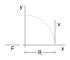
\includegraphics[width=0.7\textwidth]{01_figures/basics_cos_intuition_3}
	\captionof{figure}{Basics coordinate systems - Intuition 1}
	\label{fig:basics_cos_intuition_1}
	\vspace{5mm}
	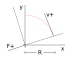
\includegraphics[width=0.7\textwidth]{01_figures/basics_cos_intuition_4}
	\captionof{figure}{Basics coordinate systems - Intuition 2}
	\label{fig:basics_cos_intuition_2}
\end{minipage}

\clearpage


Example 2 - Circular path

\begin{minipage}{0.6\textwidth}
	Applying Eq.\ref{eq:dder_r} to the body fixed coordinate system of Fig.~\ref{fig:basics_cos_intuition_3} (point mass in origin):
	\begin{align*}
		\dder{\vec{r}_0} + \dot{\vec{\omega}} \times \vec{\rho} + \vec{\omega} \times ( \vec{\omega} \times \vec{\rho}) &=  \dder{\vec{r}_0} \\
		2 \vec{\omega} \times v_{rel} &= 0 \\
		a_{rel} &= 0 \\
		\Rightarrow \dder{\vec{r}} &= \dder{\vec{r}_0}
	\intertext{Newton's law:}
		m \cdot \dder{ (\vec{r})_1 } &= \sum_i F_i = F \qquad \text{(inertial frame)}  \\
		\neq m\cdot \dder{ (\vec{r})_2} &= 0 \qquad \text{(body frame)} 
	\intertext{In the inertial frame, direction changes. In the body frame, the velocity does not change: }
		\neq m\cdot \dder{(\vec{r})_2} &= - \cosRot \times {v} + F
	\end{align*}
\end{minipage}
\begin{minipage}{0.39\textwidth}
	\centering
	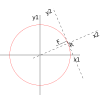
\includegraphics[width=0.8\textwidth]{01_figures/basics_cos_intuition_2}
	\captionof{figure}{Basics coordinate systems - Intuition 1}
	\label{fig:basics_cos_intuition_3}
\end{minipage}

%TODO: Absolute acceleration in rotating coordinate system. 
%TODO: Absolute acceleration in fixed coordinate system.

\clearpage
	\section{Euler Angles}

Rotation around x-axis with $\Phi$
\begin{align*}
	T(\Phi) &= \begin{pmatrix}
		1 & 0 & 0 \\
		0 & \cos{\Phi} & \sin{\Phi} \\
		0 & -\sin{\Phi} & \cos{\Phi} 
	\end{pmatrix}
\end{align*}

Rotation around y-axis with $\Theta$
\begin{align*}
T(\Theta) &= \begin{pmatrix}
\cos{\Theta} & 0 &  -\sin{\Theta}\\
0 & 1 &  \\
\sin{\Theta} & 0 & \cos{\Theta} 
\end{pmatrix}
\end{align*}

Rotation around z-axis with $\Psi$
\begin{align*}
T(\Psi) &= \begin{pmatrix}
 \cos{\Psi} & \sin{\Psi} & 0 \\
-\sin{\Psi} & \cos{\Psi} & 0 \\
         0  &         0  & 1 
\end{pmatrix}
\end{align*}

\subsection{xyz-Convention}
Orthogonal transformation matrix from inertial to body frame
\begin{align}
	\underline{T}_i^b &= \begin{pmatrix}
		\ctheta \cdot \cpsi & \ctheta \cdot \spsi & - \stheta  
		\\
		\sphi\cdot \stheta \cdot \cpsi - \cphi \cdot \spsi & \sphi \cdot \stheta \cdot \spsi + \cphi \cdot \cpsi & \sphi \cdot \ctheta 
		\\
		\cphi \cdot \stheta \cdot \cpsi +\sphi \cdot \spsi & \cphi \cdot \stheta \cdot \spsi - \sphi \cdot \cpsi & \cphi \cdot \ctheta
	\end{pmatrix} \label{eq:Tib}
\intertext{Orthogonal transformation matrix from body to inertial frame}
	\underline{T}_b^i &= \begin{pmatrix}
		\ctheta \cdot \cpsi & \sphi\cdot \stheta \cdot \cpsi - \cphi \cdot \spsi & \cphi \cdot \stheta \cdot \cpsi +\sphi \cdot \spsi
		\\
		\ctheta \cdot \spsi & \sphi \cdot \stheta \cdot \spsi + \cphi \cdot \cpsi & \cphi \cdot \stheta \cdot \spsi - \sphi \cdot \cpsi
		\\
		- \stheta  & \sphi \cdot \ctheta  & \cphi \cdot \ctheta
	\end{pmatrix} \label{eq:Tbi}
\end{align}

Karman rotation matrix. 
\begin{align}
	\omega &= \underline{T}_2^b \cdot \begin{pmatrix} \dot{\Phi}  \\ 0 \\ 0 \end{pmatrix} + \underline{T}_1^b \cdot \begin{pmatrix} 0  \\ \dot{\Theta} \\ 0 \end{pmatrix} + \underline{T}_i^b \cdot \begin{pmatrix} 0  \\ 0 \\ \dot{\Psi} \end{pmatrix} 
	\\[1em]
	\omega &= \underline{V}_i^b \cdot \dot{\vec{\Phi}} \\[1em]
	\underline{V}_b^i &= \left(\underline{V}_i^b \right)^{-1}
	\\[2em]
	\underline{V}_i^b &= \begin{pmatrix}
		1 & 0 & -\stheta 	\\
		0 & \cphi & \sphi \cdot \ctheta 	\\
		0 & -\sphi & \cphi \cdot \ctheta
	\end{pmatrix} \label{eq:Vib}
	\\[2em]
	\underline{V}_b^i &= \begin{pmatrix}
		1 & \sphi \cdot t\Theta & \cphi \cdot t\Theta 	\\
		0 & \cphi & -\sphi 	\\
		0 & \frac{\sphi}{\ctheta} & \frac{\cphi}{\ctheta}
	\end{pmatrix} \label{eq:Vbi}
\end{align}
\clearpage
	\section{Misc}

\subsection{Model linearization}
Linearization around $\vec{x}_0:~\dot{\vec{x}} = f(\vec{x}_0) + \frac{\text{d}f}{\text{d}\vec{x}} \cdot \vec{x} + \frac{\text{d}f}{\text{d}\vec{F}} \cdot \vec{F}$
\begin{align*}
\frac{\text{d}f}{\text{d} \left( \vec{x} ~~ \vec{v} \right)^T } &= 
\begin{pmatrix}
0 & 0 & 0 & \ctheta \cdot \cpsi  & \sphi \cdot \stheta \cdot \cpsi - \cphi \cdot \spsi  & \cphi \cdot \stheta \cdot \cpsi +  \sphi \cdot \spsi
\\
0 & 0 & 0 & \ctheta\cdot \spsi  & \sphi \cdot \stheta \cdot \spsi + \cphi \cdot \cpsi & \cphi \cdot \stheta \cdot \spsi - \sphi \cdot \cpsi
\\
0 & 0 & 0 & -\stheta  & \sphi \cdot \ctheta  & \cphi \cdot \ctheta 
\\
0 & 0 & 0 & 0 & r & -q
\\
0 & 0 & 0 & -r & 0 & p
\\
0 & 0 & 0 & q & -p & 0
\\
0 & 0 & 0 & 0 & 0 & 0
\\
0 & 0 & 0 & 0 & 0 & 0
\\
0 & 0 & 0 & 0 & 0 & 0
\\
0 & 0 & 0 & 0 & 0 & 0
\\
0 & 0 & 0 & 0 & 0 & 0
\\
0 & 0 & 0 & 0 & 0 & 0
\end{pmatrix} 
\\[2em]
\frac{\text{d}f}{\text{d} \vec{\Phi}} &= \begin{pmatrix} 
\left(s\Phi s\Psi + c\Phi s\Theta c\Psi \right)  v + \left(c\Phi s\Psi -s\Phi s\Theta c\Psi \right)  w & -s\Theta c\Psi u + s\Phi c\Theta c\Psi v + c\Phi c\Theta c\Psi w & - c\Theta s\Psi u + \left( - c\Phi c\Psi  -s\Phi s\Theta s\Psi \right) v + \left(s\Phi c\Psi - c\Phi s\Theta s\Psi \right) w 
\\
\left(-\sphi\cpsi + \cphi\stheta\spsi \right) v + \left( -\cphi\cpsi - \sphi\stheta\spsi \right) w & -\stheta \spsi u + \sphi\ctheta\spsi v + \cphi\ctheta\spsi w  & \ctheta\cpsi u + \left( - \cphi\spsi + \sphi\stheta\cpsi\right)v + \left(\cphi\stheta\cpsi + \sphi\spsi \right)w 
\\
\cphi\ctheta v - \sphi\ctheta w & -\ctheta u - \sphi\stheta v - \cphi\stheta w & 0  
\\
0 & g \cdot \ctheta & 0 
\\
-g \cdot \cphi \ctheta & g \cdot \sphi \cdot \ctheta & 0 
\\
g \cdot \sphi \ctheta & g \cdot \cphi \cdot \stheta & 0 
\\
-\cphi t\Theta q - \sphi t\Theta r & \frac{\sphi}{\ctheta^2} q + \frac{\cphi}{\ctheta^2} r & 0 
\\
-\sphi q- \cphi r& 0 & 0 
\\
\frac{\cphi}{\ctheta} q - \frac{\sphi}{\ctheta} r & \frac{\sphi}{\ctheta^2} \stheta q + \frac{\cphi}{\ctheta ^2 } \sphi r & 0 
\\
0 & 0 & 0 
\\
0 & 0 & 0  
\\
0 & 0 & 0  
\end{pmatrix}
\end{align*}
\begin{align*}
	\frac{\text{d}f}{\text{d} \vec{\omega}} &= \begin{pmatrix} 
		0 & 0 & 0 
	\\
		0 & 0 & 0
	\\
		0 & 0 & 0
	\\
		0 & -w & v
	\\
		w & 0 & -u
	\\
		-v & u & 0
	\\
		1 & \sphi t\Theta  & \cphi t\Theta
	\\
		0 & \cphi & -\sphi
	\\
		0 & \frac{\sphi}{\ctheta} & \frac{\cphi}{\ctheta}
	\\[0.8em]
		&\inertia^{-1} \cdot \begin{pmatrix}
			-\inertiaii{31} \cdot q + \inertiaii{21}\cdot r & 
			-\inertiaii{32} \cdot q -\inertiaii{31} \cdot p + (\inertiaii{22} - \inertiaii{33})\cdot r  & 
			\inertiaii{21}\cdot p + (\inertiaii{22}-\inertiaii{33})\cdot q + 2\cdot \inertiaii{23}\cdot r
			\\
			2\cdot \inertiaii{31}\cdot p + \inertiaii{32}\cdot q + (\inertiaii{33}-\inertiaii{11})\cdot r & 
			-\inertiaii{12} \cdot r +\inertiaii{32} \cdot p & 
			(\inertiaii{33}-\inertiaii{11})\cdot p - \inertiaii{12}\cdot q - 2\cdot\inertiaii{13}\cdot r 
			\\
			-2\cdot \inertiaii{21} \cdot p + (\inertiaii{11}- \inertiaii{22})\cdot q - \inertiaii{23}\cdot r &  
			(\inertiaii{11}-\inertiaii{22})\cdot p + 2\cdot \inertiaii{12}\cdot q + \inertiaii{13}\cdot r &
			-\inertiaii{23} \cdot p +\inertiaii{13} \cdot q
		\end{pmatrix}
	\end{pmatrix}	
	\\[2em]
	\frac{\text{d}f}{\text{d} \vec{F}} &= 
	\begin{pmatrix} 
		0 & 0 & 0 & 0 \\
		0 & 0 & 0 & 0 \\
		0 & 0 & 0 & 0 \\
		0 & 0 & 0 & 0 \\
		0 & 0 & 0 & 0 \\
		\frac{1}{m} & \frac{1}{m} & \frac{1}{m} & \frac{1}{m} \\[0.2em]
		0 & 0 & 0 & 0 \\
		0 & 0 & 0 & 0 \\
		0 & 0 & 0 & 0 \\
		 & \inertia^{-1} \cdot \begin{pmatrix}
		 	0 & l & 0 & -l \\
		 	-l & 0 &  l & 0 \\
		 	\frac{\text{d}M_1}{\text{d}F_1} & -\frac{\text{d}M_2}{\text{d}F_2} & \frac{\text{d}M_3}{\text{d}F_3} & -\frac{\text{d}M_4}{\text{d}F_4}
		 \end{pmatrix}
	\end{pmatrix}
\end{align*}


\begin{align*}
	\frac{\text{d}(-\vec{\omega} \times (\inertia\cdot\vec{\omega}))}{\text{d}\vec{\omega}} &= 
	\begin{pmatrix}
		-\inertiaii{31} \cdot q + \inertiaii{21}\cdot r & 
		-\inertiaii{32} \cdot q -\inertiaii{31} \cdot p - \inertiaii{33}\cdot r + \inertiaii{22}\cdot r & 
		-\inertiaii{33}\cdot q + \inertiaii{21}\cdot p + \inertiaii{22}\cdot q + 2\cdot \inertiaii{23}\cdot r
		\\
		-\inertiaii{11} \cdot r + 2\cdot \inertiaii{31}\cdot p + \inertiaii{32}\cdot q +\inertiaii{33}\cdot r& 
		-\inertiaii{12} \cdot r +\inertiaii{32} \cdot p & 
		-\inertiaii{11}\cdot p - \inertiaii{12}\cdot q - 2\cdot\inertiaii{13}\cdot r + \inertiaii{33}\cdot p
		\\
		-2\cdot \inertiaii{21} \cdot p - \inertiaii{22}\cdot q - \inertiaii{23}\cdot r +\inertiaii{11}\cdot q &  
		-\inertiaii{22}\cdot p + 2\cdot \inertiaii{12}\cdot q + \inertiaii{11}\cdot p + \inertiaii{13}\cdot r &
		-\inertiaii{23} \cdot p +\inertiaii{13} \cdot q
	\end{pmatrix}
	\\[1em]
	&= \begin{pmatrix}
		-\inertiaii{31} \cdot q + \inertiaii{21}\cdot r & 
		-\inertiaii{32} \cdot q -\inertiaii{31} \cdot p + (\inertiaii{22} - \inertiaii{33})\cdot r  & 
		\inertiaii{21}\cdot p + (\inertiaii{22}-\inertiaii{33})\cdot q + 2\cdot \inertiaii{23}\cdot r
	\\
		2\cdot \inertiaii{31}\cdot p + \inertiaii{32}\cdot q + (\inertiaii{33}-\inertiaii{11})\cdot r & 
		-\inertiaii{12} \cdot r +\inertiaii{32} \cdot p & 
		(\inertiaii{33}-\inertiaii{11})\cdot p - \inertiaii{12}\cdot q - 2\cdot\inertiaii{13}\cdot r 
	\\
		-2\cdot \inertiaii{21} \cdot p + (\inertiaii{11}- \inertiaii{22})\cdot q - \inertiaii{23}\cdot r &  
		(\inertiaii{11}-\inertiaii{22})\cdot p + 2\cdot \inertiaii{12}\cdot q + \inertiaii{13}\cdot r &
		-\inertiaii{23} \cdot p +\inertiaii{13} \cdot q
	\end{pmatrix}
	\\[1em]
	&\overset{\inertiaii{12}=\inertiaii{23}=0}{=} 
	\begin{pmatrix}
		-\inertiaii{31} \cdot q  & 
		-\inertiaii{31} \cdot p + (\inertiaii{22} - \inertiaii{33})\cdot r  & 
	 	(\inertiaii{22}-\inertiaii{33})\cdot q 
	\\
		2\cdot \inertiaii{31}\cdot p + (\inertiaii{33}-\inertiaii{11})\cdot r & 
		0 & 
		(\inertiaii{33}-\inertiaii{11})\cdot p  - 2\cdot\inertiaii{13}\cdot r 
	\\
	 	(\inertiaii{11}- \inertiaii{22})\cdot q  &  
		(\inertiaii{11}-\inertiaii{22})\cdot p + \inertiaii{13}\cdot r &
		\inertiaii{13} \cdot q
	\end{pmatrix}
	\\[2em]
	\inertia^{-1}\cdot \frac{\text{d}(-\vec{\omega} \times (\inertia\cdot\vec{\omega}))}{\text{d}\vec{\omega}} &\overset{\inertiaii{12}=\inertiaii{23}=0}{=} 
	\\[1em]
	&\hspace{-4.5cm}\begin{pmatrix}
		\dfrac{-\Theta_{33}\cdot \Theta_{b31} \cdot q + \Theta_{13} \cdot (\Theta_{b22}-\Theta_{b11}) \cdot q}{\Theta_{11} \cdot \Theta_{33} - \Theta^{2}_{13}} & \dfrac{\Theta_{33} \cdot (-\Theta_{b31}\cdot p + (\Theta_{b22}-\Theta_{b33}) \cdot r)+\Theta_{13} \cdot ((\Theta_{b22}-\Theta_{b11}) \cdot p - \Theta_{b33}\cdot r) }{\Theta_{11} \cdot \Theta_{33} - \Theta^{2}_{13}}  & \dfrac{\Theta_{33} \cdot (\Theta_{b22}-\Theta_{b33}) \cdot q - \Theta_{b13}^2 \cdot q  }{\Theta_{11} \cdot \Theta_{33} - \Theta^{2}_{13}} 
	\\[2em]
		\frac{1}{\Theta_{22}} \cdot \left( - \Theta_{b11} \cdot r + 2\cdot\Theta_{b31} \cdot p \right)& 0 & \frac{1}{\Theta_{22}} \cdot \left(- 2 \cdot \Theta_{b13} \cdot r + \Theta_{b33} \cdot p \right)
	\\[1em]
		\dfrac{\Theta_{13}^2 \cdot q + \Theta_{11}\cdot (\Theta_{b11} - \Theta_{b22}) \cdot q}{\Theta_{11} \cdot \Theta_{33} - \Theta^{2}_{13}} & \dfrac{\Theta_{13} \cdot (\Theta_{b31}\cdot p + (\Theta_{b33}-\Theta_{b22}) \cdot r)+\Theta_{11} \cdot ((\Theta_{b11}-\Theta_{b22}) \cdot p + \Theta_{b33}\cdot r) }{\Theta_{11} \cdot \Theta_{33} - \Theta^{2}_{13}}   & \dfrac{\Theta_{13} \cdot (\Theta_{b33}-\Theta_{b22}) \cdot q + \Theta_{b11}\cdot\Theta_{b13}\cdot q  }{\Theta_{11} \cdot \Theta_{33} - \Theta^{2}_{13}} 
	\end{pmatrix}
	\\[1.5em]
		\inertia^{-1} \cdot \vec{M} &\overset{\inertiaii{12}=\inertiaii{23}=0}{=} \begin{pmatrix}
			-\dfrac{\inertiaii{13}}{\inertiaii{11} \cdot \inertiaii{33} - \inertiaii{13}^2} \cdot \dfrac{\text{d}M_1}{\text{d}F_1} & \dfrac{\inertiaii{33}\cdot l + \inertiaii{13} \cdot \frac{\text{d}M_2}{\text{d}F_2} }{\inertiaii{11} \cdot \inertiaii{33} - \inertiaii{13}^2}  & -\dfrac{\inertiaii{13}}{\inertiaii{11} \cdot \inertiaii{33} - \inertiaii{13}^2} \cdot \dfrac{\text{d}M_3}{\text{d}F_3} & \dfrac{-\inertiaii{33}\cdot l + \inertiaii{13} \cdot \frac{\text{d}M_4}{\text{d}F_4} }{\inertiaii{11} \cdot \inertiaii{33} - \inertiaii{13}^2} 
		\\
			-\dfrac{l}{\Theta_{22}} & 0 & \dfrac{l}{\Theta_{22}} & 0
		\\
			\dfrac{\inertiaii{11}}{\inertiaii{11} \cdot \inertiaii{33} - \inertiaii{13}^2} \cdot \dfrac{\text{d}M_1}{\text{d}F_1} & \dfrac{-\inertiaii{13}\cdot l - \inertiaii{11} \cdot \frac{\text{d}M_2}{\text{d}F_2} }{\inertiaii{11} \cdot \inertiaii{33} - \inertiaii{13}^2} & \dfrac{\inertiaii{11}}{\inertiaii{11} \cdot \inertiaii{33} - \inertiaii{13}^2} \cdot \dfrac{\text{d}M_3}{\text{d}F_3} & \dfrac{\inertiaii{13}\cdot l - \inertiaii{11} \cdot \frac{\text{d}M_4}{\text{d}F_4} }{\inertiaii{11} \cdot \inertiaii{33} - \inertiaii{13}^2}
	\end{pmatrix}	
\end{align*}
\clearpage


\subsection{Inertia matrix - Inverse} \label{subsec:InertiaMatrix}

Inertia matrix
\begin{align*}
	\inertia &= \begin{pmatrix} \inertiaii{11} & \inertiaii{12} & \inertiaii{13} \\
							\inertiaii{21} & \inertiaii{22} & \inertiaii{23} \\
							\inertiaii{31} & \inertiaii{32} & \inertiaii{33} \end{pmatrix} 
\intertext{Derivation inverse}
	\det \inertia &= \inertiaii{11} \cdot \inertiaii{22} \cdot \inertiaii{33} + 2 \cdot \inertiaii{12} \cdot \inertiaii{23} \cdot \inertiaii{13} - \inertiaii{13}^{2} \cdot \inertiaii{22}-\inertiaii{23}^{2} \cdot \inertiaii{11} - \inertiaii{12}^{2} \cdot \inertiaii{33}
\intertext{Adjunct matrix}
	\inertia^{11} &= \inertiaii{22}\cdot \inertiaii{33}-\inertiaii{23}\cdot \inertiaii{32}=\inertiaii{22}\cdot \inertiaii{33}-\inertiaii{23}^{2}\\
	\inertia^{12}&=\inertiaii{21}\cdot \inertiaii{33}-\inertiaii{23}\cdot \inertiaii{31}\\
	\inertia^{13}&=\inertiaii{21}\cdot \inertiaii{32}-\inertiaii{22}\cdot \inertiaii{31}\\
	\inertia^{22}&=\inertiaii{11}\cdot \inertiaii{33}-\inertiaii{13}^{2} \\
	\inertia^{21}&=\inertiaii{12}\cdot \inertiaii{33}-\inertiaii{13}\cdot \inertiaii{23}\\
	\inertia^{23}&=\inertiaii{11}\cdot \inertiaii{32}-\inertiaii{12}\cdot \inertiaii{31}\\
	\inertia^{31}&=\inertiaii{12}\cdot \inertiaii{23}-\inertiaii{13}\cdot \inertiaii{22}\\
	\inertia^{32}&=\inertiaii{11}\cdot \inertiaii{23}-\inertiaii{13}\cdot \inertiaii{21}\\
	\inertia^{33}&=\inertiaii{11}\cdot \inertiaii{22}-\inertiaii{12}^{2} 
\\\\
	\Theta_{body, adj}^T &= \begin{pmatrix}
	\inertia^{11} & -\inertia^{21} & \inertia^{31} \\
	-\inertia^{12} & \inertia^{22} & -\inertia^{32} \\
	\inertia^{13} & -\inertia^{23} & \inertia^{33}
	\end{pmatrix}
\intertext{Inverse matrix}
	\inertia^{-1} &= \dfrac {1}{\det \inertia} \cdot \begin{pmatrix}
	\inertiaii{22}\cdot \inertiaii{33}-\inertiaii{23}^{2} & \inertiaii{13} \cdot \inertiaii{23} - \inertiaii{12}\cdot \inertiaii{13} & \inertiaii{12}\cdot \inertiaii{23}-\inertiaii{13}\cdot \inertiaii{22} 
	\\
	\inertiaii{23}\cdot \inertiaii{31}-\inertiaii{21}\cdot \inertiaii{33} & \inertiaii{11}\cdot \inertiaii{33}-\inertiaii{13}^{2} & \inertiaii{13} \cdot \inertiaii{21}-\inertiaii{11}\cdot \inertiaii{23} 
	\\
	\inertiaii{21}\cdot \inertiaii{32}-\inertiaii{22}\cdot \inertiaii{31} & \inertiaii{12}\cdot \inertiaii{31}-\inertiaii{11}\cdot \inertiaii{32} & \inertiaii{11}\cdot \inertiaii{22}- \inertiaii{12}^{2}
\end{pmatrix}
\intertext{If quadrotor is symmetric about x and y axis, $\inertiaii{12} = \inertiaii{21} = \inertiaii{23} = \inertiaii{32} = 0$ holds}
	\Rightarrow \inertia^{-1} &= \dfrac{1}{\inertiaii{11} \cdot \inertiaii{22} \cdot \inertiaii{33} - \inertiaii{22} \cdot \inertiaii{13}^2} \cdot \begin{pmatrix}
	\inertiaii{22} \cdot \inertiaii{33} & 0 		& -\inertiaii{22}\cdot \inertiaii{13} \\
	0  							   & \inertiaii{11} \cdot \inertiaii{33}-\inertiaii{13}^2 & 0 \\
	-\inertiaii{22} \cdot \inertiaii{13} & 0 		& \inertiaii{11} \cdot \inertiaii{22}
	\end{pmatrix}
	\\[1.5em]
	&= \begin{pmatrix}
	\dfrac{\inertiaii{33}}{\inertiaii{11} \cdot \inertiaii{33} - \inertiaii{13}^2} & 0 & -\dfrac{\inertiaii{13}}{\inertiaii{11} \cdot \inertiaii{33} - \inertiaii{13}^2} \\
	0  & \dfrac{1}{\inertiaii{22}} & 0 \\
	-\dfrac{\inertiaii{13}}{\inertiaii{11} \cdot \inertiaii{33} - \inertiaii{13}^2} & 0 & \dfrac{\inertiaii{11}}{\inertiaii{11} \cdot \inertiaii{33} - \inertiaii{13}^2}
	\end{pmatrix}
\end{align*}
\clearpage
\end{document}